%++++++++++++++++++++++++++++++++++++++++
% Don't modify this section unless you know what you're doing!
%\documentclass[letterpaper,12pt]{article}
\documentclass[14pt]{extarticle}
%\documentclass[journal, a4paper]{IEEEtran}
\usepackage{tabularx} % extra features for tabular environment
\usepackage{amsmath}  % improve math presentation
\usepackage{graphicx} % takes care of graphic including machinery
\usepackage[margin=1in,letterpaper]{geometry} % decreases margins
\usepackage{cite} % takes care of citations
\usepackage[final]{hyperref} % adds hyper links inside the generated pdf file
\usepackage{mathtext}
\hypersetup{
	colorlinks=true,       % false: boxed links; true: colored links
	linkcolor=blue,        % color of internal links
	citecolor=blue,        % color of links to bibliography
	filecolor=magenta,     % color of file links
	urlcolor=blue         
}
\usepackage{textcomp}
\usepackage{ gensymb }
\usepackage{latexsym}
\usepackage{geometry} % пакет для установки полей
\geometry{top=1.5cm} % отступ сверху
\geometry{bottom=2cm} % отступ снизу
\geometry{left=3cm} % отступ справа
\geometry{right=1cm} % отступ слева
\usepackage{amsfonts}
\newcommand*{\No}{\textnumero}
\renewcommand{\Re}{\mathrm{Re}}
\renewcommand{\Im}{\mathrm{Im}}

\newcommand{\const}{\mathrm{const}}
\newcommand{\arccosh}{\mathrm{arccosh}}
%++++++++++++++++++++++++++++++++++++++++

\usepackage[T2A]{fontenc}
\usepackage[utf8]{inputenc}
\usepackage[english, russian]{babel}

\hypersetup{colorlinks=true, linkcolor=black}
\begin{document}

\begin{center}
	\hfill \break
	\large{МИНОБРНАУКИ РОССИИ}\\
	\footnotesize{ФЕДЕРАЛЬНОЕ ГОСУДАРСТВЕННОЕ БЮДЖЕТНОЕ ОБРАЗОВАТЕЛЬНОЕ УЧРЕЖДЕНИЕ}\\
	\footnotesize{ВЫСШЕГО ПРОФЕССИОНАЛЬНОГО ОБРАЗОВАНИЯ}\\
	\small{\textbf{«ВОРОНЕЖСКИЙ ГОСУДАРСТВЕННЫЙ УНИВЕРСИТЕТ»}}\\
	\hfill \break
	\normalsize{Факультут Компьютерных наук}\\
	\hfill \break
	\normalsize{Кафедра Цифровых технологий}\\
	\hfill\break
	\hfill \break
	\hfill \break
	\hfill \break
	\large{Название}\\
	\hfill \break
	\hfill \break
	\hfill \break
	\normalsize{Дипломная работа\\
		\hfill \break
		02.03.01 Математика и компьютерные науки\\
		\hfill \break
		Распределенные системы и искусственный интеллект}\\
	\hfill \break
	\hfill \break
\end{center}

\hfill \break
\hfill \break

\normalsize{
	\begin{tabular}{cccc}
		Зав. кафедрой & \underline{\hspace{3cm}} &  д-р физ.-мат. наук,  проф. & С.Д. Кургалин \\\\
		Студент & \underline{\hspace{3cm}} & &А.А. Махно \\\\
		Руководитель & \underline{\hspace{3cm}}& канд. физ.-мат. наук, доц. &  А.В. Флегель \\\\
	\end{tabular}
}\\
\hfill \break
\hfill \break
\begin{center} Воронеж 2016 \end{center}
\thispagestyle{empty} % выключаем отображение номера для этой страницы

\newpage	
\tableofcontents
\thispagestyle{empty} % выключаем отображение номера для этой страницы
\newpage	
\section*{Введение}
\addcontentsline{toc}{section}{Введение}
Здесь будет введение
\newpage


\section{Физическая задача}

\begin{equation}\label{eq:input}
M_0(\epsilon, t) = \sqrt{\frac{m}{2\pi i \hbar}}\int_{-\infty}^{0} \frac{e^{i \epsilon (t - t')/\hbar}}{(t - t')^{3/2}} [e^{i S(t,t')/\hbar} - 1]dt'
\end{equation} 

\section{Описание метода перевала} 

Метод перевала применяется для оценки при больших значениях параметра $\lambda$ контурных интегралов вида
\begin{equation}\label{eq:eq6}
F(\lambda) = \int_{C}^{}\phi(t)e^{\lambda f(z)}dz
\end{equation} 
где $f(z)$ и $\phi(z)$ функции, аналитические вдоль линии интегрирования С. Интегралами вида (\ref{eq:eq6}) представляются многие специальные функции, решения дифференциальных уравнений, как обыкновенных, так и с частными производными. Эти интегралы часто встречаются при решении различных задач физики.

Рассмотрим частный случай, а именно - действительные интегралы вида

\begin{equation}\label{eq:eq7}
F(\lambda) = \int_{a}^{b}\phi(t)e^{\lambda f(t)}dt
\end{equation} 

Этот случай был рассмотрен в свое время Лапласом. Идея здесь такая. 

Предположим, что $f(t)$ имеет на отрезке $(a, b)$ один резко выраженный максимум. Чем боьше значение параметра $\lambda$, тем резче выражается этот максимум, и поэтому ясно, что при больших $\lambda$ основный вклад в значение интеграла дает окрестность точки максимума. 

В основе этого метода лежит лемма:

\textit{Лемма \label{lemma:lemma1}}: Пусть дан интеграл

$$
F(\lambda) = \int_{0}^{a}\phi(t)e^{-\lambda t^\alpha}dt \:\:\:\:\:\: (0 < a \le \infty, \alpha>0)
$$
где $\phi(t)$ при $|t|<2h$ представляется сходящимся рядом

$$
\phi(t)=t^\beta(c_0+c_1 t+\dots+c_n t^n+\dots), \; \beta>-1
$$
причем $\int_{0}^{a}|\phi(t)| e^{-\lambda_0 t^\alpha}dt\le M$ для некоторого $\lambda_0$. Тогда имеет место асимптотическое разложение

\begin{equation}\label{eq:eq8}
F(\lambda) \sim \sum_{n=0}^{\infty}\frac{c_n}{\alpha} \Gamma\left(\frac{\beta + n + 1}{\alpha}\right)\lambda^{-\frac{\beta + n + 1}{\alpha}}
\end{equation} 
где $\Gamma$ - гамма-функция Эйлера.

К доказанной лемме сводится оценка интеграла (\ref{eq:eq7})

\textit{Теорема 1\label{th:th1}}. Пусть интеграл (\ref{eq:eq7}) абсолютно сходится для некоторого $\lambda = \lambda_0$, т. е.
$$
\int_{a}^{b} |\phi(t)|e^{\lambda_0 f(t)}dt \le M,
$$
и $f(t)$ достигает своего наибольшего значения во внутренней точке $t_0$ отрезка $(а, b)$, в окрестности $| t - t_0| < \delta$ которой $f(t)$ представляется рядом
$$
f(t)=f(t_0) + a_2(t-t_0)^2+\dots+a_n(t-t_0)^n+\dots \;\; (a_2<0),
$$
причем существует $h > 0$ такое, что вне этой окрестности $f (t_0) — f(t) > h$. Пусть еще функция $t = \psi(\tau)$ определяется в окрестности точки $\tau = 0$ из уравнения $f(t_0) — f(t) = \tau^2$, причем в этой окрестности
\begin{equation}\label{eq:eq9}
\phi[\psi(\tau)]\psi^\prime(\tau) = \sum_{n=0}^{\infty} c_n\tau^n
\end{equation}

Тогда интеграл (\ref{eq:eq7}) имеет асимптотическое разложение
$$
F(\lambda)=\int_{a}^{b}\phi(t)e^{\lambda f(t)}dt \sim e^\lambda f(t_0) \sqrt{\frac{\pi}{\lambda}} \sum_{n=0}^{\infty}\frac{c_2n}{\lambda^n}\frac{(2n)!}{4^n n!}.
$$

Эта теорема относится к случаю, когда наибольшее значение $f(t)$ достигается во внутренней точке отрезка $(а, b)$. 

\textit{Теорема 2\label{th:th2}}. Пусть интеграл (\ref{eq:eq7}) абсолютно сходится для некоторого $\lambda = \lambda_0$ (см теорему 1) и $f(t)$ достигает наибольшего значения в точке $t=a$, аналитична в этой точке ($f^\prime(a) \neq 0$), и существует $h>0$ такое, что $f(a)-f(t)>h$ вне некоторой окрестности точки a. пусть еще функция $t=\psi(t)$ определяется в окрестности точки $\tau=0$ из уравнения $f(a) - f(t) = \tau$, причем в этой окрестности имеет место разложение (\ref{eq:eq9}). Тогда

\begin{equation}\label{eq:eq10}
F(\lambda) = \int_{a}^{b}\phi(t)e^{\lambda f(t)}dt \sim \frac{e^{f(a)}}{\lambda}\sum_{n=0}^{\infty}\frac{n! c_n}{\lambda^n}
\end{equation}

Суть метода перевала состоит в том, что при больших значениях параметра $\lambda$ величина интеграла

$$
F(\lambda) = \int_{C}^{}\phi(t)e^{\lambda f(z)}dz
$$
в основном определяется тем участком пути интегрирования $C$, на котором $|e^{\lambda f(z)}|=e^{\lambda \Re f(z)}$, т. е. $\Re f(z)$ велика по сравнению со значениями на остальной части $С$. При этом интеграл оценивается тем легче, чем меньше этот участок и чем круче падает величина $\Re f(z)$ В соответствии со сказанным, при применении метода перевала стараются деформировать путь интегрирования С в наиболее удобный путь $\widetilde{C}$, пользуясь тем, что по теореме Коши такая деформация не меняет величины интеграла.\cite{Lavrentyev}

Чтобы уяснить вопрос геометрически, положим $z = х + iy$ и представим
$$
u = \Re f(z)
$$
как поверхность $S$ в пространстве $(х, y, u)$. Так как функция и гармоническая, то $S$ не может иметь точек максимума и минимума, а точки, в которых $f'(z) = 0$, будут для нее точками перевала (седловыми точками, рис. \ref{ris:image2}).

\begin{figure}[h]
	\center{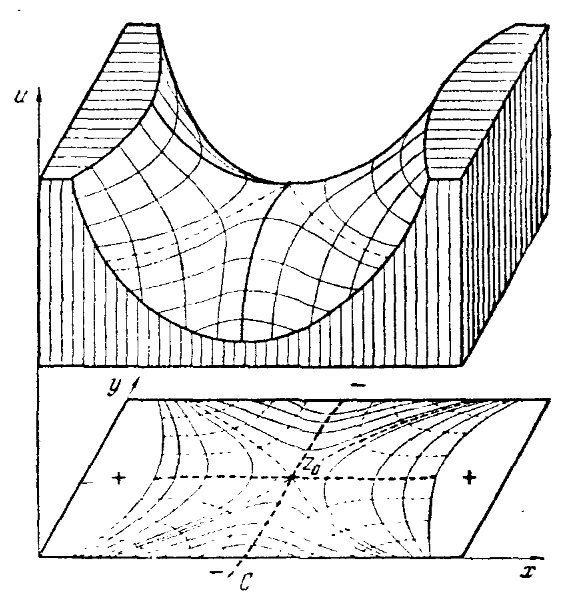
\includegraphics[width=0.3\linewidth]{pic2.png}}
	\caption{Седловые точки}
	\label{ris:image2}
	\end{figure}
	
	Наиболее удобный для оценки путь интегрирования $\widetilde{C}$, в каждой точке должен проходить в направлении наиболее быстрого изменения $\Re f(z)$, а так как функция f(z) аналитическая, то это направление должно совпадать с линией, на которой $\Im f(z) = \const$. 
	
	Также, новый контур $\widetilde{C}$ должен содержать точку $z_0$, в которой $\Re f(z)$ достигает наибольшего значения на $\widetilde{C}$. Покажем для этого случая, что $f^\prime (z_0) = 0$, то есть точка линии $\Im f(z) = \const$, в которой $\Re f (z)$ достигает наибольшего значения, является точкой перевала.
	
	Так и есть, ведь в точке $z_0$, которая является максимумом для $\Re f (z)$ производная $u=0$ вдоль линии $\widetilde{C}$ должна быть равна 0, т. е. $\frac{\partial}{\partial s}\Re f(z)=0$, а так как $\Im f(z) = \const$ на $\widetilde{C}$, то $\frac{\partial}{\partial s} \Im f(z) \equiv = 0$, а значит и 
	
	$$
	f^\prime(z_0) = \frac{\partial}{\partial s} \Re f(z) + i\frac{\partial}{\partial s} \Im f(z) = 0.
	$$ 
	
	\textit{Подведем итоги. Для метода перевала к интегралу (\ref{eq:eq6}) путь интегрирования $С$ следует деформировать в путь $\widetilde{C}$, проходящий через точку перевала $z_0$ и в окрестности этой точки идущий вдоль линии наибольшего ската $\Im f(z) = \const$ (рис. \ref{ris:image2}).}
	
	Есть одно важное обстоятельство, обеспечивающее эффективность применения метода перевала: так как вдоль линии $\widetilde{C}$ имеем $\arg e^{f(z)} = \Im f(z) = \const$, то оценка интеграла (\ref{eq:eq6}) сводится к оценке интеграла от действительной функции, которая может быть проведена по методу Лапласа для интеграла вида (\ref{eq:eq7}).  
	
	Именно это позволяет нам пользоваться полученными результатами теорем 1 и 2. 
	
	Рассмотрим  случай, когда путь интегрирования $С$ можно деформировать в путь $\widetilde{C}$, проходящий через точку перевала $z_0$, где $f^\prime(z_0) = 0$, $f^{\prime\prime}(z_0)\neq0$, и в окрестности $z_0$ совпадающий с линией наибольшего ската $\Im f(z) = \const$, причем на $\widetilde{C}$ вне этой окрестности $\Re f(z) < \Re f(z_0) - h \;(h> 0)$. Кроме того, предположим, что интеграл (\ref{eq:eq6}) абсолютно сходится для достаточно больших значений $\lambda$.
	Тогда образом, оценку интеграла можно провести на основании теоремы 1. Пусть $z = z(t)$ будет уравнение контура $\widetilde{C}$; Тогда,
	
	\begin{equation}\label{eq:eq11}
	F(\lambda) = \int_{C}^{}\phi(z) e^{\lambda f(z)}dz=e^{\lambda i \Im f[z(t)]}\int_{a}^{b}\phi[z(t)]e^{\lambda \Re f[z(t)]}z^{\prime} dt
	\end{equation}
	
	и задача сводится к оценки интеграла вида $\ref{eq:eq7}$ действительной области, разложение для которого уже было получено Лапласом, и имеет вид\cite{Lavrentyev}
	
	$$
	F(\lambda) = \int_{a}^{b}\phi(t)e^{\lambda f(t)}dt \sim \frac{e^{f(a)}}{\lambda}\sum_{n=0}^{\infty}\frac{n! c_n}{\lambda^n}
	$$
	
	Выпишем первый член этого разложения. Обозначим $\phi[z(t)]z^\prime = \widetilde{\phi}(t)$, $\Re f[z(t)] = \widetilde{f}(t)$ и тогда по формуле (\ref{eq:eq10}) получаем:
	
	\begin{equation}\label{eq:eq12}
	\int_{a}^{b} \widetilde{\phi}(t) e^{\lambda \widetilde{f}(t)}dt \sim e^{\lambda \widetilde{f}(t_0)} \sqrt{\frac{\pi}{\lambda}} \widetilde{c_0}
	\end{equation}
	где $\widetilde{c_0}$ - свободный член в разложении функции $\widetilde{\phi}[\widetilde{\psi}(\tau)]\widetilde{\psi^\prime}(\tau)$.
	
	Имеем: $\widetilde{\phi}(t_0) = \phi(z_0) z^\prime (t_0)$, и исходя из того, что $f[z(t)] = \Re f[z(t)]+ i \Im f[z(t)] = \widetilde{f}(t)+\const$ вдоль $\widetilde{C}$, то
	
	\begin{equation}\nonumber
	\widetilde{f}^{\prime\prime} (t_0) = \frac{d^2}{d t^2} f[z(t)]\;|_{t=t_0} = f^{\prime\prime} (z_0) z^{\prime^2} (t_0).
	\end{equation}
	Причем $f^\prime[z(t)] z^{\prime \prime} (t) = 0$ при $t=t_0$. Так как эта величина отрицательна, то представив $z^\prime (t_0) = k e^{i \theta}$, можно записать ее в виде $\widetilde{f}^{\prime\prime}=-|f^{\prime\prime}(z_0)| k^2$. Получаем, что 
	
	\begin{equation}\nonumber
	\widetilde{c}_0=\widetilde{\phi}(t_0) \sqrt{-\frac{2}{\widetilde{f}^{\prime\prime}(z_0)}}= \phi (z_0) e^{i \theta} \sqrt{\frac{2}{|f^{\prime\prime}(z_0)|}}
	\end{equation}
	подставим найденное значение в (\ref{eq:eq12}), а затем в (\ref{eq:eq11}), получаем искомую формулу
	
	\begin{equation}\label{eq:eq13}
	F(\lambda) \sim e^{\lambda f (z_0)}\sqrt{\frac{2\pi}{|f^{\prime \prime} (z_0)|}} \phi(z_0) e^{i \theta} \frac{1}{\sqrt{\lambda}}
	\end{equation}
	
	Как уже много раз говорилось, точка $z_0$ - это точка, где $\Re f(z)$ достигает своего максимального значения. В то же время совершенно обычная ситуация - когда на искомом контуре $\widetilde{C}$ имеется несколько точек перевала, в которых значения $\Re f (z)$ находятся вблизи к наибольшему, то следует взять сумму выражений (\ref{eq:eq13}) по всем этим точками. 
	
	Тот случай, когда контур интегрирования заканчивается в точке перевала $z_0$, аналогичным образом приводится к теореме \ref{th:th2}.
	
	Итак, мы получили рабочую формулу, подставляя в которую составляющие наших искомых функций $\phi (z)$ и $f (z)$, мы должны получать приближенные значения интеграла, когда $\lambda \rightarrow \infty$ 

\newpage
\section{Численное решение}

Выполним численное интегрирование интеграла (\ref{eq:input})

Заметим, что нижний предел интегрирования у нас $-\infty$. Очевидно, что с этими производить вычисления невозможно, но зато наша начальная функция под первым интегралом

$$
A(t) = -c\int_{-\infty}^{t} F(\tau) d\tau
$$

Имеет вид:

\begin{equation}\label{eq:A_eval}
F(t) =  F_0 e^{ -\frac{x^2}{\alpha^2} }  \cos(\omega x)
\end{equation}

и является затухающей. Таким образом, решив уравнение 

$$
|e^{ -\frac{t_b^2}{\alpha^2} }| < \epsilon
$$

на промежутке $[-\infty; 0]$, приближаясь слева, мы получим то самое значение $t_b$, при котором можно не учитывать отрезок интегрирования в связи с достижением необходимой точности.

В этом случае интеграл (\ref{eq:A_eval}) примет вид:

$$\label{eq:easy}
A(t) = -c\int_{t_b}^{t} F(\tau) d\tau
$$

Для вычисления этого интеграла воспользуемся методом интегрирования Гаусса, когда 

$$
\int_{x_1}^{x_2} f(x) dx = \sum_{j=1}^{N} \omega_j f(x_j)
$$

В методе Гаусса точки интегрирования берутся с разными интервалами и при этом имеют различные веса $\omega_i$, характеризующие их вклад в интеграл.

Метод Гаусса также может считать интегралы от неограниченных, быстро затухающий функция. Нам это не потребуется, но в связи с тем, что у нас этот интеграл (\ref{eq:A_eval}) будет входить, далее, в подынтегральные функции, а также с необходимостью на каждом шаге пересчета матричного элемента, менять пределы интегрирования придется использовать адаптивные методы, то есть с переменным шагом. Они не так сложны в реализации, но поскольку вычислений будет очень много, имеет смысл воспользоваться уже готовой библиотекой GNU GSL. 

GNU GSL - Это библиотека, написанная на языке программирования C для численных вычислений в прикладной математике и науке.

Самый главный ее плюс - в скорости вычислений, а также относительная экономия памяти, или же по крайней мере, ограничение ее использования. А также в ней реализовано огромное количество численных методов

Нас пока что интересует только один из них, а именно $gsl\_integration\_qags$, позволяющий нам интегрировать функцию на отрезке с заданной точностью. 

Стоит отменить, что для первого интеграла (\ref{eq:A_eval}) GSL не смог добиться точности абсолютной ошибки выше $10^{-13}$, а значит, использовать результат в дальнейшем с большей точностью смысла не имеет.

Далее, у нас есть интеграл $\alpha$

\begin{equation}\label{eq:alpha}
	\alpha(\epsilon, t, t') = \frac{|e|}{c} [A_{\tau}(\epsilon) - \frac{1}{(t-')}\int_{t'}^{t}A(\tau) d\tau]
\end{equation}

Который потом будет входить в интеграл 

\begin{equation}\label{eq:s_integrate}
	S(t, t') = -\frac{1}{2m}\int_{t'}^{t} \alpha(\epsilon, t, t')^2 d\epsilon
\end{equation}

Для упрощения вычислений имеет преобразовать функцию (\ref{eq:s_integrate}) к виду

\begin{equation}\label{eq:s_integrate2}
S(t, t') = -\frac{1}{2m}\int_{t'}^{t} A(\tau)^2 d\tau + \frac{1}{2(t'-t)} \int_{t'}^{t}A(\tau) d\tau
\end{equation}

Итак мы получили функцию $S(t, t')$, которая входит в исходный интеграл ($\ref{eq:input}$). Но сложность для вычислений представляет именно последний интеграл $M$

Заметим схожесть интеграла ($\ref{eq:input}$) с общим видом преобразования Фурье

Введем замену $t - t' = \tau$, получаем

$$
M = \int_{0}^{\infty}\frac{e^{i\epsilon \tau}}{{\tau}^{3/2}}(e^{i [+ S(t, t-\tau)]/\hbar} - 1) d\tau 
$$
$$
F(\xi) = \int_{-\infty}^{\infty}e^{i\xi \tau} F(\tau) d\tau 
$$

Для дискретного преобразования Фурье разницы между нашими пределами не будет, так как функция будет определена только на отрезке [0; $t_{end}$].
То есть интегрирование можно ускорить, использовав не стандартные методы интегрирования, а используя дискретное преобразование Фурье. Или же быстрое преобразование Фурье, что будет еще лучшим решением.

Для этого воспользуемся библиотекой FFTW.

$FFTW$ является набором модулей на языках Си и Фортран для вычисления быстрого преобразования Фурье (БПФ). FFTW позволяет работать как с действительными, так и с комплексными числами, с произвольным размером входных данных, т.е. с длиной данных, не обязательно являющейся числом, кратным $2^n$. Библиотека также включает модули параллельной обработки БПФ, которые позволяют использовать ее на многопроцессорных машинах с общей и распределенной памятью.





%Который легко интегрируется методом Гаусса.
%



\section{Формулы}
Дана формула (\ref{eq:input})

Часть интеграла с (-1) может быть отброшена, так как (говорилось ранее) основной вклад с интеграл вносят седловые точки. !!!!!Написать что-нибудь еще

$$
M \sim \int_{-\infty}^{t} \frac{1}{(t-t')^{3/2}} e^{i[\epsilon (t - t') + S(t, t')]/\hbar} dt'
$$

Введем замену $t - t' = \tau$, получаем

$$
M \sim \int_{0}^{\infty}\frac{1}{{\tau}^{3/2}}e^{i [\epsilon \tau + S(t, t-\tau)]/\hbar} d\tau
$$

Если обозначить
$
f(t, \tau) = \epsilon \tau + S(t, t-\tau) 
$ и
$
\phi(\tau) = \frac{1}{{\tau}^{3/2}} 
$

То получим формулу вида

$$
M \sim \int_{0}^{\infty} \phi(\tau) e^{i f(t, \tau)/\hbar} d\tau
$$

Которая совпадает с формулой для Метода Перевала, применимого для интегралов вида

$$
\int_{-\infty}^{\infty} \phi(x) e^{f(x)}dx
$$

Для нашего случая приближение должно принимать вид:

$$
M_0(\epsilon, t) \simeq \sqrt{\frac{m}{2\pi i \hbar}}\sum_{t0}e^{f(t_0)} \sqrt{-\frac{2}{f''(t_0)}} \phi(t_0)
$$, где $t_0$ - корни уравнения $f'(t) = 0$

Остается только получить формулу для $f''(t)$ и решить уравнение на стационарные точки 

В формулу (\ref{eq:input}) входят некоторые элементы, такие как

$$
S(t, t') = -\frac{1}{2m}\int_{t'}^{t} \alpha(\epsilon, t, t')^2 d\epsilon
$$

$$
\alpha(\epsilon, t, t') = \frac{|e|}{c} [A_{\tau}(\epsilon) - \frac{1}{(t-')}\int_{t'}^{t}A(\tau) d\tau]
$$

$$
A(t) = -c\int_{-\infty}^{t} F(\tau) d\tau
$$

Найдем теперь перевальные точки ($t_0$), дифференцируя по $\tau$

$$
f(t, \tau) = \epsilon \tau + S(t, t-\tau),
$$
$$
f'(t, \tau) = \epsilon + S'(t, t-\tau)
$$
\begin{equation}\label{eq:points}
	f'(t, \tau)=0 => S'(t, t-\tau) = -\epsilon
\end{equation}

С введенной заменой $S$ примет вид

$$
S(t, t-\tau) = -\frac{1}{2m}\int_{t-\tau}^{t} \alpha(\epsilon, t, t-\tau)^2 d\epsilon
$$

Дифференцируя по $\tau$, получаем

$$
S'(t, t-\tau) = -\frac{1}{2m} \alpha(t-\tau, t, t-\tau)^2
$$

Произведем обратную замену $t_0 = t-\tau$ и с учетом того, что $S' = -\epsilon$ (\ref{eq:points}), получаем явный вид уравнения на стационарные точки:

$$
\alpha(t_0, t, t_0) = 2 \epsilon m
$$

Теперь найдем $f''(t)$

$$
f''(t) = -\frac{1}{2m}[\alpha(t-\tau, t, t-\tau)^2]' =
$$

$$
= -\frac{2\alpha(t_0, t, t_0)}{2m} * \alpha(t_0, t, t_0)'
$$

Рассмотрим новое $\alpha$

$$
\alpha(t_0, t, t_0) = \frac{|e|}{c} [A_{\tau}(t_0) - \frac{1}{(t-t_0)}\int_{t_0}^{t}A(\tau) d\tau]
$$

%Продифференцируем первую часть ($A_\tau(\epsilon)$) по $t_0$:

%$$
%A'(t_0) = (-c\int_{-\infty}^{t} F(\tau) d\tau)' =
%$$

%$$
%= cF(t_0)
%$$

%И вторую ($\frac{1}{(t-t_0)}\int_{t_0}^{t}A(\tau) d\tau$):

%$$
%\frac{\partial[\frac{1}{t-t_0}\int_{t_0}^{t}A(\tau)d\tau]}{\partial t_0} = -\frac{1}{(t - t_0)^2} \int_{t_0}^{t}A(\tau)d\tau - A(t_0) \frac{1}{t-t_0}
%$$

Итого, получаем формулу для $F''$ вида

$$
F''(t, t_0) = -\frac{|e|\alpha(t_0, t, t_0)}{m} [F(t_0) - 
$$
$$
-\frac{1}{(t - t_0)^2} \int_{t_0}^{t}A(\tau)d\tau - A(t_0) \frac{1}{t-t_0}]
$$

Обозначим $D = - 2 m F''(t, t_0)$ и $$S^\sim = \epsilon \tau + S(t, t-\tau) = \epsilon(t-t_0) + S(t, t_0)$$

Подставляя в формулу для Метода перевала, получаем:

$$
M_0(\epsilon, t) \simeq \sqrt{\frac{m}{2\pi i \hbar}}\sum_{t_0}\frac{e^{\frac{i}{\hbar}S^\sim(t, t_0)} \sqrt{2m}}{\sqrt{D} (t-t_0)^{3/2}} = \frac{1}{\sqrt{\pi i \hbar}}\sum_{t_0}\frac{me^{\frac{i}{\hbar}S^\sim(t, t_0)} }{\sqrt{D} (t-t_0)^{3/2}}
$$

\section*{Заключение}
\addcontentsline{toc}{section}{Заключение}
  

 
\newpage
\bibliographystyle{utf8gost705u}  %% стилевой файл для оформления по ГОСТу
\bibliography{biblio}     %% имя библиографической базы (bib-файла) 
\end{document} 